\chapter{Présentation des cas tests}
\label{sec:ann_exemples}

\section{Équations scalaires couplées}

On rappelle le problème \eqref{pb:edo_partic_1}: \\
{\itshape{}Pour $\epsilon$ donné, trouver $x\in C^{\infty}([0,T]; \R$ et $z \in C^{\infty}([0,T])$ telles que} 
\begin{equation} \label{pb:ann_edo_partic_1}
\left\{ \begin{array}{l}
\dot{x} = -x^3(z-z^3/3) \vphantom{\displaystyle\sum_0} , \\ \displaystyle
\dot{z} = -\inveps z + x(1-z^2/2) 
\end{array} \right. 
\qquad \text{et} \qquad 
\left\{ \begin{array}{l}
x(0) = x_0 = 0,8 \vphantom{\displaystyle\sum_0} \\
z(0) = z_0 = 0,05 .
\end{array} \right.
\end{equation}
Traçons la solution de ce système sur $[0; 0,7]$ pour diverses valeurs de $\epsilon$. 
\begin{figure}[!h]
\centering
\includegraphics[width=.9\textwidth]{img/ann/solution_cas1.eps}
\caption{Solution $x$ (à gauche) et $z$ (à droite) du problème \eqref{pb:ann_edo_partic_1} sur $[0; 0,7]$, avec en pointillé l'approximation de la variété associée.}
\end{figure}

Il est apparent sur la figure qu'on a en temps long $\dot{x} = \O(\epsilon)$. 
On voit aussi très clairement $z_{\infty} = \O(\epsilon)$. 



\section{Oscillations lentes de $x$}

On rappelle le problème \eqref{pb:edo_partic_2}: \\
{\itshape{}Pour $\epsilon$ donné, trouver $x \in C^{\infty}([0,T];\R^2)$ et $z \in C^{\infty}([0,T]; \R)$ telles que} 
\begin{equation} \label{pb:ann_edo_partic_2}
\left\{ \begin{array}{l}
\dot{x} = (1-z)\begin{pmatrix} 0 & -1 \\ 1 & 0 \end{pmatrix} x , \\ \displaystyle
\dot{z} = \inveps z + x_1^2 x_2^2 \vphantom{\displaystyle\sum^0}
\end{array} \right. 
\qquad \text{et} \qquad 
\left\{ \begin{array}{l}
x(0) = x_0 = \begin{pmatrix} 0,1 \\ 0,7 \end{pmatrix} , \\
z(0) = z_0 = 0,05 . \vphantom{\displaystyle\sum^0}
\end{array} \right.
\end{equation}
On ne trace pas la solution en fonction du temps, mais plutôt son parcours dans $\R^3$. 
\begin{figure}[!h]
\centering
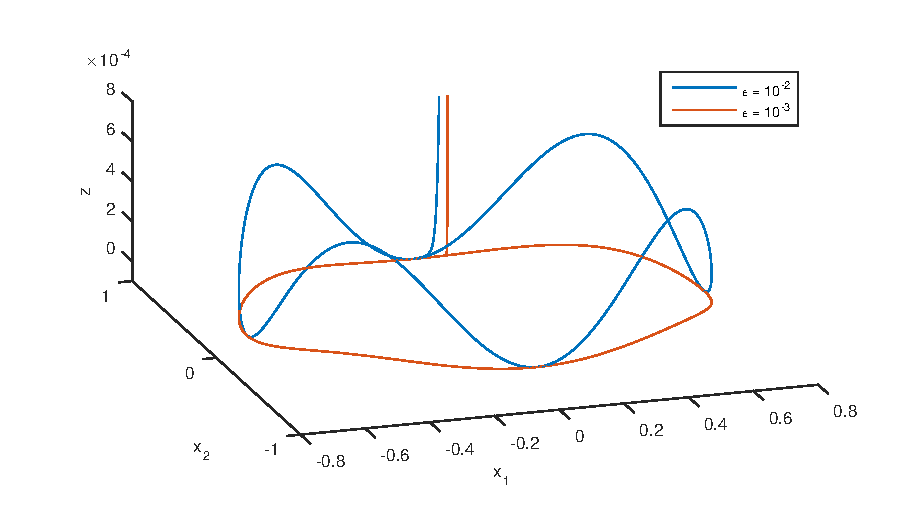
\includegraphics[width=.9\textwidth]{img/ann/solution_cas2.eps}
\caption{Parcours de $(x_1,x_2,z)$ dans $\R^3$ où $x,z$ sont solutions du problème \eqref{pb:ann_edo_partic_2} sur $[0; 10]$.}
\end{figure}

Le système semble converger rapidement vers un système périodique où $x_1,x_2$ et $z$ oscillent. 
On trace $z$ pour vérifier que la période ne dépend qualitativement pas de $\epsilon$.

\begin{figure}[!h]
\centering
\includegraphics[width=.8\textwidth]{img/ann/solution_z_cas2.eps}
\caption{Solution $z$ du problème \eqref{pb:ann_edo_partic_2} sur $[0; 3]$ pour $\epsilon = 10^{-2},10^{-3}$.}
\end{figure}
En effet sur la variété on a $\dot{x} = \begin{pmatrix}
0 & -1 \\ 1 & 0 
\end{pmatrix} x + \O(\epsilon)$, ce qui cause l'oscillation de $x_1,x_2$. 
Le terme dominant pour déterminer la période est donc forcément indépendant de $\epsilon$. 